\section{Ujicoba dan Analisis}

\subsection{Uji coba Kebenaran}
Uji coba kebenaran dilakukan dengan cara mengumpulkan berkas kode implementasi kedalam daring penilaian online SPOJ. Studi kasus yang diselesaikan adalah \textit{The Bytelandian Cryptographer(Act IV)} dengan code CRYPTO4. Hasil uji kebenaran dan waktu eksekusi program pada situs SPOJ ditunjukkan pada gambar \ref{fig:best}.
\begin{figure}[H]
\centering
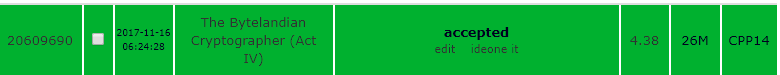
\includegraphics[scale=0.3]{images/best.png}
\caption{Hasil uji kebenaran dengan melakukan submission ke situs penilaian daring SPOJ}
\label{fig:best}
\end{figure}

Uji coba kinerja dari implementasi program yang dihasilkan dengan cara mengumpulkan berkas kode implementasi kedalam daring penilaian online SPOJ sebanyak 30 kali dengan mencatat waktu dan memori yang dibutuhkan, dapat dilihat pada gambar \ref{fig:asf} dan table \ref{tab:statistik}.
\begin{figure}[H]
\centering
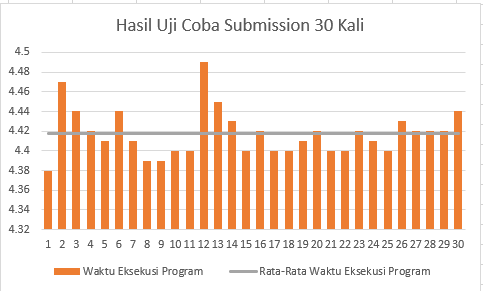
\includegraphics[scale=0.4]{images/uji31.png}
\caption{Hasil Uji Coba Submission ke situs penilaian daring SPOJ sebanyak 30 kali}
\label{fig:asf}
\end{figure}
\begin{table}[H]
	\centering
	\caption{Kecepatan Maksimal, Minimal, dan Rata-Rata dari Hasil Uji Coba Pengumpulan 30 Kali pada Situs Pengujian Daring Spoj}	
	\begin{tabular}{|l|l|} \hline
		Waktu Maksimal & $ 4,49 $ detik\\ \hline
		Waktu Minimal & $ 4,38 $ detik\\ \hline
		Waktu Rata-Rata & $ 4.418 $ detik\\ \hline
		Memori Maksimal & $ 27 $ MB\\ \hline
		Memori Minimal & $ 26 $ MB\\ \hline
		Memori Rata-Rata & $ 26.5 $ MB\\ \hline
	\end{tabular}
	
	\label{tab:statistik}
\end{table}


\subsection{Analisa Kompleksitas}
Berdasarkan algoritma yang telah dibentuk pada bagian metode penyelesaian maka, didapatkan algoritma dengan kompleksitas waktu $\mathcal{O}(T*\frac{M}{2}*(N+S))$ 
	Dimana $n$ adalah panjang karakter \textit{plaintext} atau \textit{ciphertext} , $\frac{M}{2}$ adalah batas atas kunci dibagi dengan 2, $N$ adalah jumlah posisi karakter yang terdapat pada tahap 2 pada subbab \ref{chap:selesai}, dan $S$ adalah jumlah posisi karakter yang terdapat pada tahap 1 pada subbab \ref{chap:selesai}. Pada kondisi \textit{worst case} $T*(N+S)=1.000.000$, sedangakan $\frac{M}{2}$ adalah $50.000$. Hasilnya $50$ miliar perulangan, dengan asumsi $1$ detik adalah $1$ miliar perulangan, maka waktu yang dibutuhkan adalah $50$ detik. Oleh karena itu hal ini tidak mungkin bisa dilakukan begitu saja. Diperlukan pruning pada sumber kode yang ada untuk memangkas waktu eksekusi program. \textit{Prunning} yang dapat dilakukan ketiga menggunakan \textit{Kasiski Examination} dan \textit{Intersection}. Apabila semuanya ini telah dilakukan pasti mendapatkan seperti gambar \ref{fig:best} pada daring online SPOJ.
